\chapter{How to Use a Journal}

This lecture begins where enthusiasm usually breaks down. A listener hears an inspiring seminar, buys a journal, opens it, and is met not by insight but by blank pages. From that small crisis the lecture develops a disciplined method. We begin with the journal as an object that must be chosen and carried, move to writing as a way of separating ourselves from confusion, widen to the capture and ordering of ideas, and end with review, communication, imagination, and legacy. The mathematics is therefore heuristic rather than scientific. It gives the lecture a visible spine: vague experience is written, writing creates distance, distance permits analysis, and analysis returns to life as action.

\section{Blank Pages, Ownership, and the Habit of Beginning}

The lecture opens with a string of questions that anyone who has bought an empty notebook will recognize. What are we supposed to write? Should it be personal, businesslike, or both? How often should we use it? What kind of book should it be? Even the little anxieties appear: does spelling count? The opening move is important. We do not begin with a doctrine about the journal; we begin with the obstacle that prevents the journal from being used at all.

The first answer is practical. A journal is \emph{your} book. It is not a standardized instrument that arrives with its use already determined. Size, binding, paper, portability, lines or blank pages, and even the sensory pleasure of holding it all matter because they govern whether the book will be opened often enough to become part of life.

The lecture gives this thought almost as a proportional law:
\begin{equation}
\operatorname{Use}(J)\propto \operatorname{Feel}(J).
\end{equation}
Here \(J\) denotes the journal as a working object. The point is not quantitative precision; the point is that use rises and falls with felt suitability.

A cautious standard reconstruction of the same claim is
\begin{equation}
\operatorname{Effectiveness}(J)=f(\text{fit},\text{comfort},\text{portability},\text{habit}).
\end{equation}

That compression gathers together several remarks in the lecture: the journal should be pleasant enough to invite return, large enough to receive thought, but small enough to travel. This is why the lecture warns against a beautiful but immobile book. A journal that does not fit the briefcase, desk, or day will be left at home, gathering dust instead of observations.

At the same time, the lecture does not turn the search for the right journal into a perfectionist ritual. Over the years methods change. Loose-leaf systems, file cards, cheap notebooks, hardbound volumes, lined pages, blank pages: all may serve a genuine need for a season. Flexibility is itself named as a key to success. But flexibility is not hesitation. In the beginning, the lecture insists, one thing matters more than system:
\[
\text{first success}=\text{the formation of the journal habit}.
\]

That habit is defined less by volume than by availability. The first discipline is to have the journal with us.

\section{What Goes into a Journal? Writing as Clarification and Problem Solving}

Only after the object has been discussed does the lecture announce its main pivot: buying a journal is easy; filling it is the real challenge. At this point the question becomes not what shape the journal has, but what work it is to perform.

\subsection{Question \& Answer}

The natural question is: \emph{What should go into a journal if it is to have meaning and value in life?}

The lecture answers by changing the terms of the question. We are not first given a list of permitted subjects. Instead, we are told to consider the purposes and functions of a journal. Once the \emph{why} of writing becomes clear, the \emph{what} becomes much less mysterious.

The first major function is that the journal helps us figure things out: life, people, business dilemmas, and most of all ourselves. The lecture's basic process may be written as
\begin{equation}
\text{vague problem}\rightarrow \text{written description}\rightarrow \text{factual picture}\rightarrow \text{actionable adjustment}.
\end{equation}

This is immediately condensed by the lecture into a stronger operational claim:
\begin{equation}
\text{write problem}\rightarrow \text{discover ways of making it right}.
\end{equation}

The reason is not mystical, though the lecture briefly speaks of something magical in writing down a problem. What writing actually does is create distance. A difficulty merely carried in the mind is mixed with fear, hurry, hope, memory, and imagination. Once written, it becomes an object we can inspect. The lecture says that writing creates a space between us and the problem, and within that space solutions have room to grow.

We can formalize that update as
\begin{equation}
\text{mental picture}_{n+1}=R\!\left(\text{written account}_{n}\right),
\end{equation}
where \(R\) denotes rereading. The next picture is formed not from the old confusion alone, but from the written account that has been externalized and re-examined.

\begin{figure}[h]
\centering
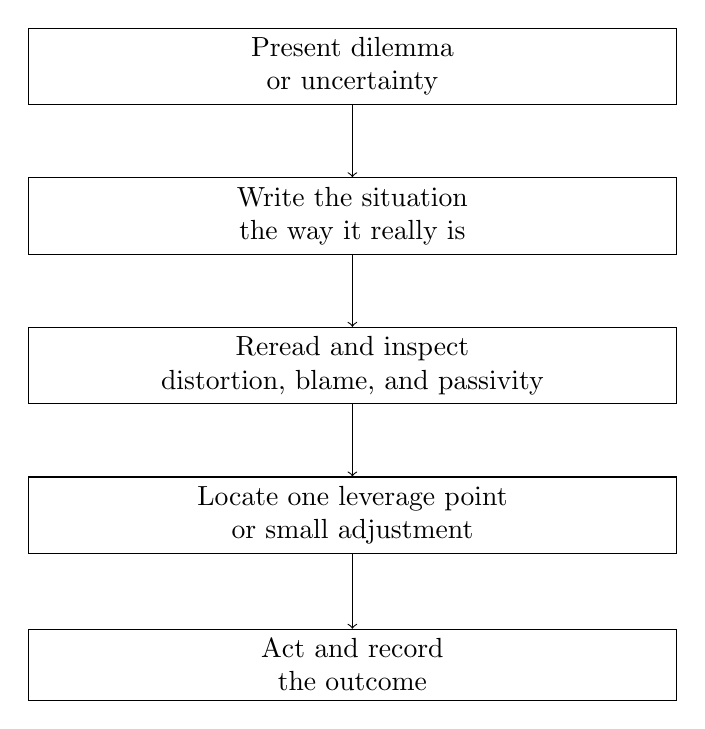
\begin{tikzpicture}
\node[draw, align=center, text width=8cm] (a) at (0,0) {Present dilemma\\or uncertainty};
\node[draw, align=center, text width=8cm] (b) at (0,-1.9) {Write the situation\\the way it really is};
\node[draw, align=center, text width=8cm] (c) at (0,-3.8) {Reread and inspect\\distortion, blame, and passivity};
\node[draw, align=center, text width=8cm] (d) at (0,-5.7) {Locate one leverage point\\or small adjustment};
\node[draw, align=center, text width=8cm] (e) at (0,-7.6) {Act and record\\the outcome};
\draw[->] (a) -- (b);
\draw[->] (b) -- (c);
\draw[->] (c) -- (d);
\draw[->] (d) -- (e);
\end{tikzpicture}
\caption{A transcript-backed schematic of the lecture's first journal cycle.}
\end{figure}

This is why the lecture recommends that one of the first entries may simply be a current dilemma. It may be personal, business, family, or financial. We are not told to wait until we have something literary to say. We are told to begin where life is already pressing.

\section{Distortion, Responsibility, and the Weak Point}

But writing the problem is only the first step. The lecture immediately slows down and says so. The next step is to analyze what has been written. Here the journal ceases to be a therapeutic blur and becomes a disciplined instrument.

The sequence of analysis is explicit. First, look for exaggeration or distortion. Are we really telling it as it is? Perhaps concern has made the situation look worse than it is, or enthusiasm has made it look better. Second, look for the tendency to blame circumstances or other people. Third, look for passive hope: the expectation that others or the surrounding world must change before our own problem can be solved. Finally, look for the weak point in the obstacle.

\paragraph{Worked update rule.}
Let \(P\) be a present problem and let \(W_k(P)\) denote the \(k\)-th written revision of its statement. Then the lecture's procedure may be represented as
\begin{align}
W_0(P)&=\text{first telling of the problem},\\
W_1(P)&=\text{remove exaggeration or unwarranted optimism},\\
W_2(P)&=\text{remove blame shifted to circumstances or other people},\\
W_3(P)&=\text{remove passive hope and identify one controllable adjustment},\\
O(P)&=\text{record the eventual outcome}.
\end{align}

The significance of this little chain is easy to miss. The lecture is not proposing that writing replace action. It is proposing that writing refine the statement of the case before action is chosen. Better thinking comes before better acting.

At the center of this section stands one of the lecture's main maxims:
\begin{equation}
\text{things get better when you get better}.
\end{equation}

This is the direct rejection of passive hope. Circumstances may be real and difficult, but waiting for them to repair themselves is not a method. The lecture presses the point again with a second maxim:
\begin{equation}
\text{major problem}\approx \text{few minor adjustments in attitude or action plan}.
\end{equation}

This is framed through the David and Goliath image and through the metaphor of the microscope. We are asked to look at the problem as a scientist might look at an organism on a slide, through what the lecture calls the microscope of truth. Once the shape, perimeter, and composition of the problem become visible, leverage becomes possible.

The lecture then adds the part many people would omit: record the conclusion. If the chosen action worked, it becomes something we can remember. If it failed, it becomes something we must remember. An error repeated is more costly than an error made once and learned from. The journal is therefore a record not merely of feeling, but of correction.

\section{Commitment Now and the Capture of Ideas}

At this point the lecture changes key. A suggestion may be good, even obviously good, and still come to nothing if it is deferred. The enemy is the word ``sometime.'' The lecture's transition is sharp because it wants to prevent admiration from substituting for decision.

A compressed version of that warning is
\begin{equation}
\text{intent}\not\Rightarrow \text{accomplishment}.
\end{equation}

The lecture's advice is concrete: if the suggestion has merit, do not promise vaguely to try it later. Make a commitment, open the journal, and write at least one page. The point is not rhetorical severity for its own sake. The lecture wants to force the first act, because without the discipline to begin there will be no discipline to continue.

From this pressure the lecture opens its second major function: the capture of good ideas. A good line, an interesting conversation, a business detail, a personal discovery, an observation from a sermon or seminar---all of these are easily admired and just as easily lost. The church anecdote matters precisely because it stages this difference. Hundreds of people hear the sermon, but only one person is writing.

The central inequality is straightforward:
\begin{equation}
\text{information captured now}>\text{fragments remembered later},
\end{equation}
and the corresponding reinforcement claim is
\begin{equation}
\text{idea on paper}\rightarrow \text{etched more firmly in consciousness}.
\end{equation}

This is the lecturer's argument for seriousness. To hear or read is one thing. To stop, write, and preserve is another. The journal is the tool by which we become, in the lecture's phrase, serious students.

The lecture then extends the time horizon. Many captured ideas will not yet have a use. They are still worth saving. Later, when conflict or opportunity arrives, the armory assembled in quieter times may become immediately serviceable. Capture now, use later: that is the rhythm.

\section{From Fragments to Knowledge: Organization, Review, and Patterns}

Yet capture alone is not enough. If the page becomes another version of the cluttered mental drawer, it will store value without making value available. The lecture therefore moves from accumulation to order.

Its constructive metaphor is memorable:
\begin{equation}
\text{snowflakes}\rightarrow \text{blocks}\rightarrow \text{structure},
\end{equation}
and then more explicitly,
\begin{equation}
\text{good ideas in one area}\rightarrow \text{solid block},\qquad
\text{solid blocks}\rightarrow \text{whole new life}.
\end{equation}

The point is not decorative imagery. Small pieces, if gathered by theme, come to bear weight. But what cannot be found cannot be used. The lecture's counter-image is the extra drawer in a desk or kitchen: filled with useful things, but arranged so chaotically that nothing is retrievable when needed.

For this reason the journal becomes a storage system. The lecture gives concrete index-style examples:
\begin{align}
\text{Financial Ideas}&\mapsto \{5,53,96,104\},\\
\text{Ideas for Increasing Company Efficiency}&\mapsto \{46,82,111\}.
\end{align}

The experiments with multiple journals, multiple colors of ink, and finally reserved sections inside a single volume show the same practical principle. What matters is not one universally perfect scheme, but the existence of a scheme:
\begin{equation}
\text{capture}+\text{organization}+\text{review}\rightarrow \text{practical knowledge}.
\end{equation}

The lecture then announces what it calls the key point: journals attain their greatest value when they are reviewed. Writing is only the first half of the operation:
\begin{equation}
\text{writing}=\text{capture},\qquad
\text{re-reading}=\text{translation of information into practical knowledge}.
\end{equation}

This is where self-discovery enters. Rereading does not merely remind us of what happened. It reveals what we consistently notice, what we omit, and what kind of person appears between the lines. The lecture offers the example of a woman who discovered, on rereading, that her journal centered almost entirely on other people's lives. That omission was itself a revelation.

To make such pattern detection easier, the lecture recommends that each entry carry date, time, and location. We may write this as
\begin{equation}
M=(\text{date},\text{time},\text{location}).
\end{equation}

This small addition turns the journal into something almost experimental. The lecture gives a worked example. A man notices that Wednesday afternoon and evening entries repeatedly contain discouragement and self-doubt. He checks the exceptions, finds the recurrent luncheon association, and identifies the source.

\paragraph{Worked example: the Wednesday pattern.}
Let the \(n\)-th entry carry metadata \(M_n=(d_n,t_n,\ell_n)\). The lecture's example becomes
\begin{align}
d_n=\text{Wednesday},\qquad t_n=\text{afternoon or evening}
&\Longrightarrow \text{recurrent discouragement},\\
\text{trace the pattern to a repeated luncheon association}
&\Longrightarrow \text{identify the hidden cause},\\
\text{remove or revise the association}
&\Longrightarrow \text{the pattern weakens or disappears}.
\end{align}

This leads naturally to one of the lecture's strongest conceptual relations:
\begin{equation}
\text{cause}\rightarrow \text{effect},
\end{equation}
and therefore
\begin{equation}
\text{external event}\rightarrow \text{written description}\rightarrow \text{inner understanding}.
\end{equation}

Events happen outside us, but unless they are described clearly they remain confused within us. The lecture pushes this still further into emotion. Writing about fear, pain, or concern gives those feelings a page to inhabit instead of letting them remain an indistinct pressure in the mind:
\begin{equation}
\text{powerful negative emotion}\xrightarrow{\text{writing}}\text{diminished strength}.
\end{equation}

A nearby sentence in the transcript about positive emotion is unstable, so the safest interpretation is the one the lecture immediately clarifies: writing reduces the grip of fear, while the deliberate capture of excitement can stabilize and intensify it.

\section{Communication, Frequency, and the Inward Decision}

From review and self-discovery the lecture broadens again. The journal does not only help us know ourselves. It also trains us to communicate. First, it gives us a place to speak to ourselves and hear what we are actually saying. Then, because inward description becomes clearer, outward description improves as well.

A compact form of the claim is
\begin{equation}
\text{clearer self-description}\rightarrow \text{clearer communication with others}.
\end{equation}

This comes in two stages. First, we learn to translate what is happening around us into terms we can understand. Second, we learn to express what is happening within us in terms the world can understand. The lecture lingers over the difficulty of this. Technology may have improved channels of communication, but human beings are still separated by the opacity of private thought. The journal is proposed as practice in crossing that distance.

The lecture also insists that effective communication across outward difference rests on inward commonality. We may differ in age, education, status, profession, or circumstance, but sorrow, joy, fear, need, and hope remain recognizably human. By recording how life has felt to us at different moments, we become better prepared to understand how it may feel to someone else.

\subsection{Question \& Answer}

At this stage the lecture raises another natural question: \emph{How often should we be writing?}

The answer is balanced rather than rigid. As often as we wish and as often as we need. But two extremes are rejected. Never writing means participating in life without capturing it. Constant writing means capturing life without participating in it. The lecture compresses its answer into a useful formula:
\begin{equation}
\text{life}=\text{observation}+\text{action}.
\end{equation}

The journal belongs on the side of observation, but not as the rival of action. This is why the lecture returns once more to the simplest discipline: always have it with us. One may not open it for weeks, but to carry it is already to present oneself to life as a conscious observer and participant.

The closing pressure of this section returns to agency:
\begin{equation}
\text{decision}+\text{action}\ \text{must come from inside you}.
\end{equation}

No tape, no seminar, no external encouragement can replace that interior source. The anecdote about the audience of nearly five hundred listeners, only a few of whom were actually keeping journals months later, shows the gap between being impressed and being changed. Admiration is common. Practice is rare.

\section{Imagination, Goals, and Legacy}

The lecture's final movement enlarges the journal one last time. If we are still having difficulty writing, one of the first entries may simply be an explanation of why we bought the journal in the first place. That small suggestion turns out to be important, because it makes the journal answer to a specific need: to express, analyze, ponder, explain, record, consider, or examine some part of life. There is no single correct procedure. Journals are as open as the lives that use them.

From there the lecture moves beyond record into design. The journal becomes a place to author life in advance. We are asked to place ourselves in imagined circumstances, describe what an ideal job, relationship, income, code of conduct, or lifestyle would look like, and then convert those mental pictures into structured commitments.

The constructive sequence is one of the lecture's cleanest:
\begin{equation}
\text{dreams}\rightarrow \text{written goals with priorities and deadlines}\rightarrow \text{detailed plan of action}.
\end{equation}

This is the moment at which the journal ceases to be merely archival. It becomes projective. What is first imagined is then written; what is written is then ordered; what is ordered can then be acted upon.

Two quoted maxims appear here in equation-like form:
\begin{equation}
\text{conceive}+\text{believe}\Rightarrow \text{achieve},
\end{equation}
and
\begin{equation}
\text{thinketh}\rightarrow \text{becomes}.
\end{equation}

These should remain visibly marked as quoted maxims rather than treated as original laws of the lecture. Their purpose is to sharpen the final transition: what is created on the page is not meant to remain there. Under belief, commitment, discipline, and desire, it seeks embodiment in life.

The lecture ends by extending the journal beyond private usefulness. Journals capture hopes, sorrows, lessons, friendships, disappointments, and achievements, and in doing so they preserve the knowledge of a single lifetime. The closing citation from the Durants widens this into inheritance. Civilization is not simply received. It is learned, earned, gathered, and transmitted. On this view the journal is one of the small instruments by which personal history becomes part of collective heritage.

\section{Summary}

The lecture unfolds as a single deliberate chain. The journal is first chosen so that it may actually be used. It is then used to write a present problem, and writing creates the distance in which correction becomes possible. Analysis removes distortion, blame, and passive hope, and directs attention toward a leverage point. Ideas are captured before they evaporate, organized before they are lost, and reviewed before they harden into dead storage. Events, feelings, causes, and recurring patterns are tied together. Communication improves because inner description becomes more exact. Finally, imagination is written into goals, and goals into plans. The journal thus becomes at once an instrument, a memory, a mirror, a bridge, and a design table for life.